\documentclass[
 size=14pt,
 paper=smartboard,  % a4paper, smartboard, screen
 mode=present, 		% present, handout, print
 display=slides, 	% slidesnotes, notes, slides
 style=tuliplab,  	% TULIP Lab style
 pauseslide,
 fleqn,leqno]{powerdot}{}

\usepackage{courier}
\usepackage{graphicx}
 %%==========================================================================================
\input{mod-preamble}
%%==========================================================================================

% title
% TODO: Customize to your Own Title, Name, Address
%
\title{Scientific Writing}
\author{
Shu Li
\\
\\School of Information Technology
\\Deakin University, Australia
}
\date{\gitCommitterDate}


% Customize the setting of slides
\pdsetup{
% TODO: Customize tlhe left footer, and right footer
rf=\href{http://www.tulip.org.au}{
Last Changed by: \textsc{\gitCommitterName}\ \gitVtagn-\gitAbbrevHash\ (\gitAuthorDate)
},
cf={Scientific Writing},
}

\begin{document}

\maketitle
%%==========================================================================================

\begin{slide}[toc=,bm=]{Overview}
\tableofcontents[content=currentsection,type=1]
\end{slide}

%%==========================================================================================
\section{Introduction}

%%%%%%%%%%%%%%%%%%%%%%%%%%%%%%%%%%%%%%%%%%%%%%%%%%%%%%%%%%%%%%%%%%%%%

\begin{slide}[toc=,bm=]{The purpose of your paper is...}
	\begin{figure}[htbp]
	    
\includegraphics[width=0.5\linewidth]{./figures/writing-skills/purpose.eps}
	\end{figure}
\end{slide}

%%%%%%%%%%%%%%%%%%%%%%%%%%%%%%%%%%%%%%%%%%%%%%%%%%%%%%%%%%%%%%%%%%%%%

\begin{slide}[toc=,bm=]{The purpose of your paper is...}
    \begin{itemize}
    	\item In science and engineering, the purpose is proposing a feasible method to a research problem and justfying the contributions theoretically and experimentally
    	\begin{itemize}
		    \item A research problem
		    \item Research motivation
		    \item Research gap
		    \item Method to solve the problem
		    \item Experimental results to prove the effectiveness of the method
		    \item Contributions
	    \end{itemize}
	\end{itemize}
\end{slide}

%%%%%%%%%%%%%%%%%%%%%%%%%%%%%%%%%%%%%%%%%%%%%%%%%%%%%%%%%%%%%%%%%%%%

\begin{slide}[toc=,bm=]{What are readers?}
\twocolumn[
lcolwidth=0.5\linewidth,
rcolwidth=0.45\linewidth
]
{
	\begin{itemize}
		\item The most important readers are
			\begin{itemize}
				\item Reviewers!!!	
			\end{itemize}
		\item What reviewers look for? 
			\begin{itemize}
				\item Readers have expectations when they read, and the most effective way to write is to fulfill their expectations.
			\end{itemize}
	\end{itemize}
}
{	
	\begin{figure}	
		
\includegraphics[width=\linewidth]{./figures/writing-skills/reviewers.eps}
	\end{figure}
}	
\end{slide}

%%%%%%%%%%%%%%%%%%%%%%%%%%%%%%%%%%%%%%%%%%%%%%%%%%%%%%%%%%%%%%%%%%%%%

%%==========================================================================================
\section{Before writing}

%%%%%%%%%%%%%%%%%%%%%%%%%%%%%%%%%%%%%%%%%%%%%%%%%%%%%%%%%%%%%%%%%%%%%

\begin{slide}[toc=,bm=]{Some questions you should have in mind before writing}
	\begin{itemize}
		\item If you can answer these questions very clearly, then you can start writing your paper.
		\begin{itemize}
			\item \textcolor{orange}{Research Problem}
				\begin{itemize}
					\item The problem to be investigated
				\end{itemize}
			\item \textcolor{orange}{Related Work}
				\begin{itemize}
					\item The existing solutions
				\end{itemize}
			\item \textcolor{orange}{Research Gaps}
				\begin{itemize}
					\item The challenges/limits/barriers of the research problem (3-4 challenges)
				\end{itemize}
			\item \textcolor{orange}{Rationale}
				\begin{itemize}
					\item Why could the proposed approach avoids these challenges
				\end{itemize}	
			\item \textcolor{orange}{Contribution}
				\begin{itemize}
					\item Clearly state contributions corresponding to the challenges above	
				\end{itemize} 		
		\end{itemize}
	\end{itemize}	
\end{slide}

%%%%%%%%%%%%%%%%%%%%%%%%%%%%%%%%%%%%%%%%%%%%%%%%%%%%%%%%%%%%%%%%%%%%%

\begin{slide}[toc=,bm=]{Ways of writing in Tulip Lab}
	\begin{itemize}
		\item Generallly, 
			\begin{itemize}
				\item Firstly, complete a conference paper, then extend into a journal paper.
			\end{itemize}
		\item \textcolor{orange}{In Tulip Lab}
			\begin{itemize}
				\item Firstly, set higher goals - a journal paper
				\item Orders of writing
					\begin{itemize}
						\item PowerPoint/slides (Clarify structure and argument of the paper)
						\item Journal paper (Full version of the research content)
						\item Conference paper (More specific research point)
					\end{itemize}
			\end{itemize}
	\end{itemize}	
\end{slide}

%%%%%%%%%%%%%%%%%%%%%%%%%%%%%%%%%%%%%%%%%%%%%%%%%%%%%%%%%%%%%%%%%%%%%

\begin{slide}[toc=,bm=]{What is better before writing?}
	\begin{itemize}
		\item Select similar 1\~{}2 articles as templates 
			\begin{itemize}
				\item Papers from a different area are better to prevent plagiarism
			\end{itemize}	
	\end{itemize}	
\end{slide}

%%%%%%%%%%%%%%%%%%%%%%%%%%%%%%%%%%%%%%%%%%%%%%%%%%%%%%%%%%%%%%%%%%%%

\begin{slide}[toc=,bm=]{When do you start writing?}
	\begin{itemize}
		\item Begin to write mannuscipt when the algorithm and the experiments are clear. 
		\item The algorithm performance and experimental results can be adjusted in the process of writing.
		\item However, some terms such as the proposed algorithm name and notations about relevant data must be determined.
			\begin{itemize}
				\item Algorithm name need to be catchy: \texttt{FPDZxs}, for example, is not as catchy as \texttt{Fredos}.
			\end{itemize}		
	\end{itemize}	
\end{slide}

%%%%%%%%%%%%%%%%%%%%%%%%%%%%%%%%%%%%%%%%%%%%%%%%%%%%%%%%%%%%%%%%%%%%%

%%==========================================================================================
\section{Structure of a paper}

%%%%%%%%%%%%%%%%%%%%%%%%%%%%%%%%%%%%%%%%%%%%%%%%%%%%%%%%%%%%%%%%%%%%%

\begin{slide}[toc=,bm=]{Stereotyped writing}
\twocolumn[lcolwidth=0.4\linewidth,
rcolwidth=0.6\linewidth
]
{
	\begin{itemize}
		\item Title and Authors
		\item Abstract
		\item Introduction
		\item Related Work
		\item Methods and Rationale
		\item Experimental Results
		\item Conclution
		\item References		
	\end{itemize}
	}
{
	\begin{figure}	
		
\includegraphics[width=0.5\textwidth]{./figures/writing-skills/stereotypedwriting.eps}
	\end{figure}
}
\end{slide}

%%%%%%%%%%%%%%%%%%%%%%%%%%%%%%%%%%%%%%%%%%%%%%%%%%%%%%%%%%%%%%%%%%%%%

\begin{slide}[toc=,bm=]{Methodology}
	\begin{itemize}
		\item If this paper is about a new method/technique/algorithm developed, write its novel aspects in great detail. 
		\item After the method section completed, ask yourself following questions
			\begin{itemize}
				\item Are all new terms defined? 
				\item If you read this section for the first time, do you have enough information to reproduce all the work?
			\end{itemize}
		\item The terms should be consistent throughout the paper.
			\begin{itemize}
				\item For example, \texttt{attributes}, \texttt{factors}, \texttt{variables}, \texttt{features} are all fine, but you can only choose one in a paper.
			\end{itemize}
	\end{itemize}	
\end{slide}

%%%%%%%%%%%%%%%%%%%%%%%%%%%%%%%%%%%%%%%%%%%%%%%%%%%%%%%%%%%%%%%%%%%%%

\begin{slide}[toc=,bm=]{Experimental Results}
	\begin{itemize}
		\item The more experiments you can find or design, the more likely your work will be accepted and used by others.
		\item Data unrelated to the central theme should not be included in the paper because they will only confuse readers.
	\end{itemize}	
\end{slide}

%%%%%%%%%%%%%%%%%%%%%%%%%%%%%%%%%%%%%%%%%%%%%%%%%%%%%%%%%%%%%%%%%%%%%

\begin{slide}[toc=,bm=]{Title}
	\begin{itemize}
		\item The title can advertise your methods, your results, or the implications of your results.
		\item A title is the paper in one sentence. Put the most important, sexy information in your title. 
		\item Two annoying titles
			\begin{itemize}
				\item ...based...
				\item Including self-created algorithm name that only you can understand
			\end{itemize}
	\end{itemize}	
\end{slide}

%%%%%%%%%%%%%%%%%%%%%%%%%%%%%%%%%%%%%%%%%%%%%%%%%%%%%%%%%%%%%%%%%%%%

\begin{slide}[toc=,bm=]{Introduction}
	\begin{itemize}
		\item The first sentence: link the first sentence to the title of the paper
		\item The first paragraph
			\begin{itemize}
				\item Some of the terms used in the title
				\item The field of research and its importance
			\end{itemize}
		\item The second paragraph
			\begin{itemize}
				\item A critical survey of the field: solution, or partial solution, the existing unsolved problem, the difficulties or barriers
			\end{itemize}
		\item The third paragraph
			\begin{itemize}
				\item The challenges addressed by the proposed solution in details
			\end{itemize}
	\end{itemize}	
\end{slide}

%%%%%%%%%%%%%%%%%%%%%%%%%%%%%%%%%%%%%%%%%%%%%%%%%%%%%%%%%%%%%%%%%%%%

\begin{slide}[toc=,bm=]{Related Work}
	\begin{itemize}
		\item The existing solutions in this field, and the challenges.
			\begin{itemize}
				\item Important representative works
				\item The latest research achievement 
			\end{itemize}		
		\item Summary those works, not just list every paper.
		\item Related Work is important because it help you identify the research gap, datasets, and evaluation criteria.	
		\item In experiment results, you maybe compare your methods with the state-of-the-art approaches to achieve the better results.
	\end{itemize}	
\end{slide}

%%%%%%%%%%%%%%%%%%%%%%%%%%%%%%%%%%%%%%%%%%%%%%%%%%%%%%%%%%%%%%%%%%%%

\begin{slide}[toc=,bm=]{Conclution}
	\begin{itemize}
		\item Separate the results from their interpretations, implications and conclusion
			\begin{itemize}
				\item Start with a review of results obtained and their interpretations 
				\item Various trials and tests done, the effects of parameter changes on results, comparisons to other studies, problems yet to be solved, future or on-going work
			\end{itemize}
	\end{itemize}	
\end{slide}

%%%%%%%%%%%%%%%%%%%%%%%%%%%%%%%%%%%%%%%%%%%%%%%%%%%%%%%%%%%%%%%%%%%%%

\begin{slide}[toc=,bm=]{Abstract}
	\begin{itemize}
		\item The importance of the subject area (linked backward to title)
		\item The problem to be investigated
		\item The uniqueness of your approach 
		\item The significance
		\item Implications and impact of the results
	\end{itemize}	
\end{slide}

%%%%%%%%%%%%%%%%%%%%%%%%%%%%%%%%%%%%%%%%%%%%%%%%%%%%%%%%%%%%%%%%%%%%

\begin{slide}[toc=,bm=]{Authors}
	\begin{itemize}
		\item CS General Practise
			\begin{itemize}
				\item The person who came up with the problem/the idea is \textcolor{orange}{the first author}. 
				\item Other people who do the experiments, wirte the paper, even if write completely, can only be other authors, maybe second.
			\end{itemize}
		\item \textcolor{orange}{In Tulip Lab}
			\begin{itemize}
				\item The first author is the one who writes the paper even if the question/idea/experiment are put forward by someone else's.
				\item Generally, if a tuliplab member completes his/her experiment and paper writing, he/she will be the first author in most cases.
				\item The authors are all contributors to the paper, maybe including the fund supporter of the paper.
			\end{itemize}
	\end{itemize}
\end{slide}

%%%%%%%%%%%%%%%%%%%%%%%%%%%%%%%%%%%%%%%%%%%%%%%%%%%%%%%%%%%%%%%%%%%%%

%%%%%%%%%%%%%%%%%%%%%%%%%%%%%%%%%%%%%%%%%%%%%%%%%%%%%%%%%%%%%%%%%%%%

\begin{slide}[toc=,bm=]{Summary}
	\begin{itemize}
		\item Rather than a indepenent section from each other, the sections in the article are related each other, and gadually bring the essence of the paper from begining to the end to form a story.
			\begin{itemize}
				\item Introduction section defines challenges and research issues of the paper.
				\item Related Work section further summarizes challenges and research issues.
				\item The rationale and methodology of the paper is aimed at these issues.
				\item Experiments are designed for each issue.
				\item Every issue should have its own contribution.		
			\end{itemize}
	\end{itemize}
\end{slide}

%%%%%%%%%%%%%%%%%%%%%%%%%%%%%%%%%%%%%%%%%%%%%%%%%%%%%%%%%%%%%%%%%%%%%

%%==========================================================================================
\section{Readers' expectations}

%%%%%%%%%%%%%%%%%%%%%%%%%%%%%%%%%%%%%%%%%%%%%%%%%%%%%%%%%%%%%%%%%%%%

\begin{slide}[toc=,bm=]{Readers' expectation for a sentence}
	\begin{itemize}
		\item Readers expect familiar information at the beginning of a sentence.
			\begin{itemize}
				\item \textcolor{mygreen!50}{The accuracy of the model structures is given by TM-score. In case of a perfect match to 3experimental structure, TM-score would be 1.}
				\item \textcolor{orange}{The accuracy of the model structures is measured by TM-score, which is equal to 1 if there is a perfect match to experimental structure.}
			\end{itemize}
		\item The golden rule for writing the start of a sentence is to ask yourself this question: have I introduced this concept before?	
	\end{itemize}
\end{slide}

%%%%%%%%%%%%%%%%%%%%%%%%%%%%%%%%%%%%%%%%%%%%%%%%%%%%%%%%%%%%%%%%%%%%

\begin{slide}[toc=,bm=]{Readers' expectation for a sentence}
	\begin{itemize}
		\item Readers expect the action verb immediately after the subject.
			\begin{itemize}
				\item \textcolor{mygreen!50}{The smallest URFs (URFA6L), a 207-nucleotide (nt) reading frame overlapping out of phase the NH2-terminal portion of the adenosinetrip hosphatase (ATPase) subinit 6 gene has been identified as the animal equivalent of the recently discovered yeast H+-ATPase subunit 8 gene.}
				\item \textcolor{orange}{The smallest of the URFs is URFA6L, a 207-nucleotide (nt) reading frame overlapping out of phase the NH2-terminal portion of the adenosinetriphosphatase (ATPase) subinit 6 Gene; it has been identified as the animal equivalent of the recently discovered yeast H+-ATPase subunit 8 gene.}
			\end{itemize}
		\item It is much better to have a short subject followed immediately by a verb and long object.	
	\end{itemize}
\end{slide}

%%%%%%%%%%%%%%%%%%%%%%%%%%%%%%%%%%%%%%%%%%%%%%%%%%%%%%%%%%%%%%%%%%%%

\begin{slide}[toc=,bm=]{Readers' expectation for a sentence}
	\begin{itemize}
		\item Readers expect that each sentence makes only one point, which is emphasized at the end of the sentence.
			\begin{itemize}
				\item \textcolor{mygreen!50}{The enthalpy of hydrogen bond formation between the nucleoside bases 2-deoxyguanosine (dG) and 2-deoxycytidine (dC) has been determined by direct measurement.}
				\item \textcolor{orange}{We have directly measured the enthalpy of hydrogen bond formation between the nucleoside bases 2-deoxyguanosine (dG) and 2-deoxycytidine (dC).}
			\end{itemize}
		\item Each sentence makes only one point, which is emphasized at the end of the sentence. It also avoids the “large head and small foot” problem.	
	\end{itemize}
\end{slide}

%%%%%%%%%%%%%%%%%%%%%%%%%%%%%%%%%%%%%%%%%%%%%%%%%%%%%%%%%%%%%%%%%%%%

\begin{slide}[toc=,bm=]{Readers’ expectations of a paragraph}
	\begin{itemize}
		\item Each paragraph should only tell one story about one subject.
	\end{itemize}
\end{slide}

%%%%%%%%%%%%%%%%%%%%%%%%%%%%%%%%%%%%%%%%%%%%%%%%%%%%%%%%%%%%%%%%%%%%

\begin{slide}[toc=,bm=]{Readers’ expectations of a table/figure}
	\begin{itemize}
		\item It is expected that more familiar \(old\) information in the left and new information on the right.
	\end{itemize}

\twocolumn[lcolwidth=0.4\linewidth,
rcolwidth=0.4\linewidth
]
{
	\begin{table}
	\fontsize{11pt}{11pt}\selectfont
	\setlength{\abovecaptionskip}{0pt}
	\setlength{\belowcaptionskip}{12pt}
	\centering
	\caption{Sample 1}
		\begin{tabular}{c|c}
				\toprule
				 \textbf{Temp($^\circ$C)} & \textbf{Time} \\ 
				\midrule
				 25  & 0 \\
				 27  & 3 \\
				 29  & 6 \\
				 32  & 12 \\
				 32  & 15 \\
				\bottomrule
		\end{tabular}
	\end{table}
}
{
	\begin{table}
	\fontsize{11pt}{11pt}\selectfont
	\setlength{\abovecaptionskip}{0pt}
	\setlength{\belowcaptionskip}{12pt}
	\centering
	\caption{\textcolor{orange}{Sample 2}}
		\begin{tabular}{c|c}
				\toprule
				 \textbf{Time} & \textbf{Temp($^\circ$C)}\\ 
				\midrule
				 0  & 25 \\
				 3  & 27 \\
				 6  & 29 \\
				 12  & 32 \\
				 15  & 32 \\
				\bottomrule
		\end{tabular}
	\end{table}
}
\end{slide}

%%%%%%%%%%%%%%%%%%%%%%%%%%%%%%%%%%%%%%%%%%%%%%%%%%%%%%%%%%%%%%%%%%%%

\begin{slide}[toc=,bm=]{Readers’ expectations of a table/figure}
	\begin{itemize}
		\item Another rule for tables is to save the best for the last.
	\end{itemize}
	\begin{table}
	\fontsize{11pt}{11pt}\selectfont
	\setlength{\abovecaptionskip}{0pt}
	\setlength{\belowcaptionskip}{12pt}
	\centering
	\caption{Sample 3}
		\begin{tabular}{c|c|c|c|c}
				\toprule
				 Benchmark & SALIGN & Lindahl & PROSPECTOR 3 & LiveBench 8\\ 
				 \midrule
				 SPARKS & 53.1\% & 325.9 & 529.0 & 38.3 \\
				 SPARKS2 & 54.9\% & 341.0 & 591.0 & 40.7 \\
				 \textcolor{orange}{This work} & \textcolor{orange}{56.6\%} & \textcolor{orange}{349.2} & \textcolor{orange}{601.9} & \textcolor{orange}{42.2} \\
				\bottomrule
		\end{tabular}
	\end{table}
\end{slide}

%%%%%%%%%%%%%%%%%%%%%%%%%%%%%%%%%%%%%%%%%%%%%%%%%%%%%%%%%%%%%%%%%%%%

\begin{slide}[toc=,bm=]{Readers’ expectations of a table/figure }
	\begin{itemize}
		\item Use solid lines for your work and dashed lines for other studies. 
		\item Symbols are mixed with open and filled from top to bottom to maximize the difference between various curves. 
		\item Spell out the titles for X and Y axes (rather than short-hands).
	\end{itemize}
	\begin{figure}	
		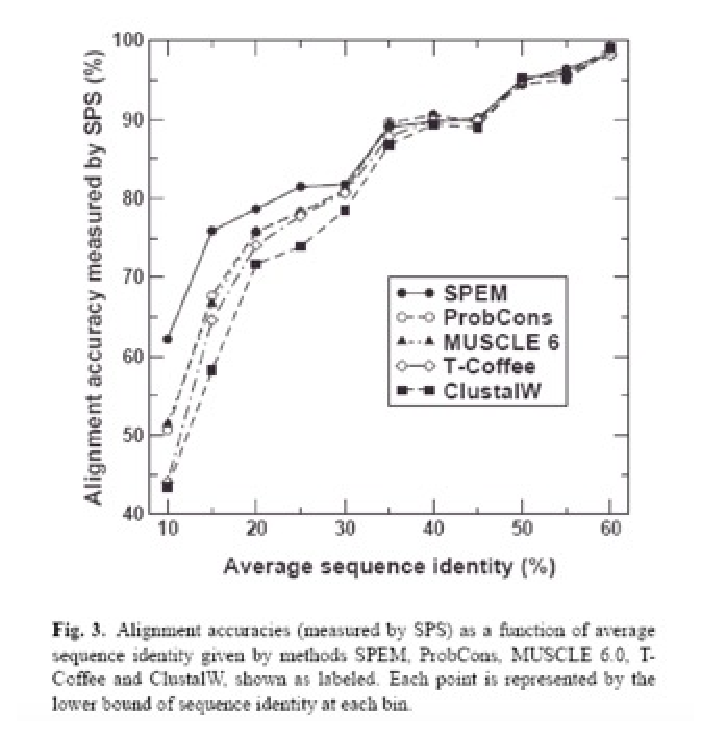
\includegraphics[scale=0.6]{./figures/writing-skills/figure-expectation.eps}
	\end{figure}
\end{slide}

%%%%%%%%%%%%%%%%%%%%%%%%%%%%%%%%%%%%%%%%%%%%%%%%%%%%%%%%%%%%%%%%%%%%%

%%==========================================================================================
\section{Tools}

%%%%%%%%%%%%%%%%%%%%%%%%%%%%%%%%%%%%%%%%%%%%%%%%%%%%%%%%%%%%%%%%%%%%

\begin{slide}[toc=,bm=]{Writing Tools}
	\begin{itemize}
		\item \href{http://www.phrasebank.manchester.ac.uk}{Academic phrasebank (\emph{www.phrasebank.manchester.ac.uk})}
		\item \href{http://latexqc.ieee.org/}{Latex check (\emph{{latexqc.ieee.org}})}
		\item English Writing check 
			\begin{itemize}
				\item  \href{https://app.grammarly.com/}{Grammerly (\emph{{app.grammarly.com}})}
		    	\item  \href{http://www.netspeak.org/}{Netspeak (\emph{{www.netspeak.org}})}
		    	\item  \href{http://linggle.com/}{Linggle (\emph{{linggle.com}})}
		    	\item  \href{https://github.com/amperser/proselint} {Proselint (\emph{{proselint.com}})}
		    \end{itemize}
	\end{itemize}

	\begin{figure}	
		\subfigure{
			\includegraphics[width=0.4\textwidth]{./figures/writing-skills/linggle.eps}}
		\subfigure{
			\includegraphics[width=0.4\textwidth]{./figures/writing-skills/netspeak.eps}
		}
	\end{figure}
\end{slide}

%%%%%%%%%%%%%%%%%%%%%%%%%%%%%%%%%%%%%%%%%%%%%%%%%%%%%%%%%%%%%%%%%%%%%

\begin{slide}[toc=,bm=]{Academic Accounts}
	\begin{itemize}
		\item As a researcher, you must maintain your academic accounts so that other researchers can find you and see your research achievements.
			\begin{itemize}
				\item  \href{https://orcid.org/}{ORCID (\emph{{orcid.org}})}
		    	\item  \href{https://scholar.google.com/intl/en/scholar/citations.html}{Google Scholar (\emph{{scholar.google.com}})}
		    \end{itemize}
	\end{itemize}
\end{slide}

%%%%%%%%%%%%%%%%%%%%%%%%%%%%%%%%%%%%%%%%%%%%%%%%%%%%%%%%%%%%%%%%%%%%%

\begin{slide}[toc=,bm=]{\LaTeX~  Template}
	\begin{itemize}
		\item As a member in Tulip Lab, you should get familiar with tuliplab's templatex
			\begin{itemize}
				\item  \href{https://github.com/tulip-lab/templatex}{\LaTeX~ template (\emph{{https://github.com/tulip-lab/templatex}})}
		    \end{itemize}
	\end{itemize}
\end{slide}

%%%%%%%%%%%%%%%%%%%%%%%%%%%%%%%%%%%%%%%%%%%%%%%%%%%%%%%%%%%%%%%%%%%%%

\begin{slide}[toc=,bm=]{Git Repository}
	\begin{itemize}
		\item In Tulip Lab, a paper idea, no matter how many conferences or journals it contributes to, has only one git repository.			
	\end{itemize}
\end{slide}

% %%%%%%%%%%%%%%%%%%%%%%%%%%%%%%%%%%%%%%%%%%%%%%%%%%%%%%%%%%%%%%%%%%%%%

%%==========================================================================================
\section{After Writing}

% %%%%%%%%%%%%%%%%%%%%%%%%%%%%%%%%%%%%%%%%%%%%%%%%%%%%%%%%%%%%%%%%%%%%%

\begin{slide}[toc=,bm=]{TULIP Paper Submission Procedure}
	\centering
	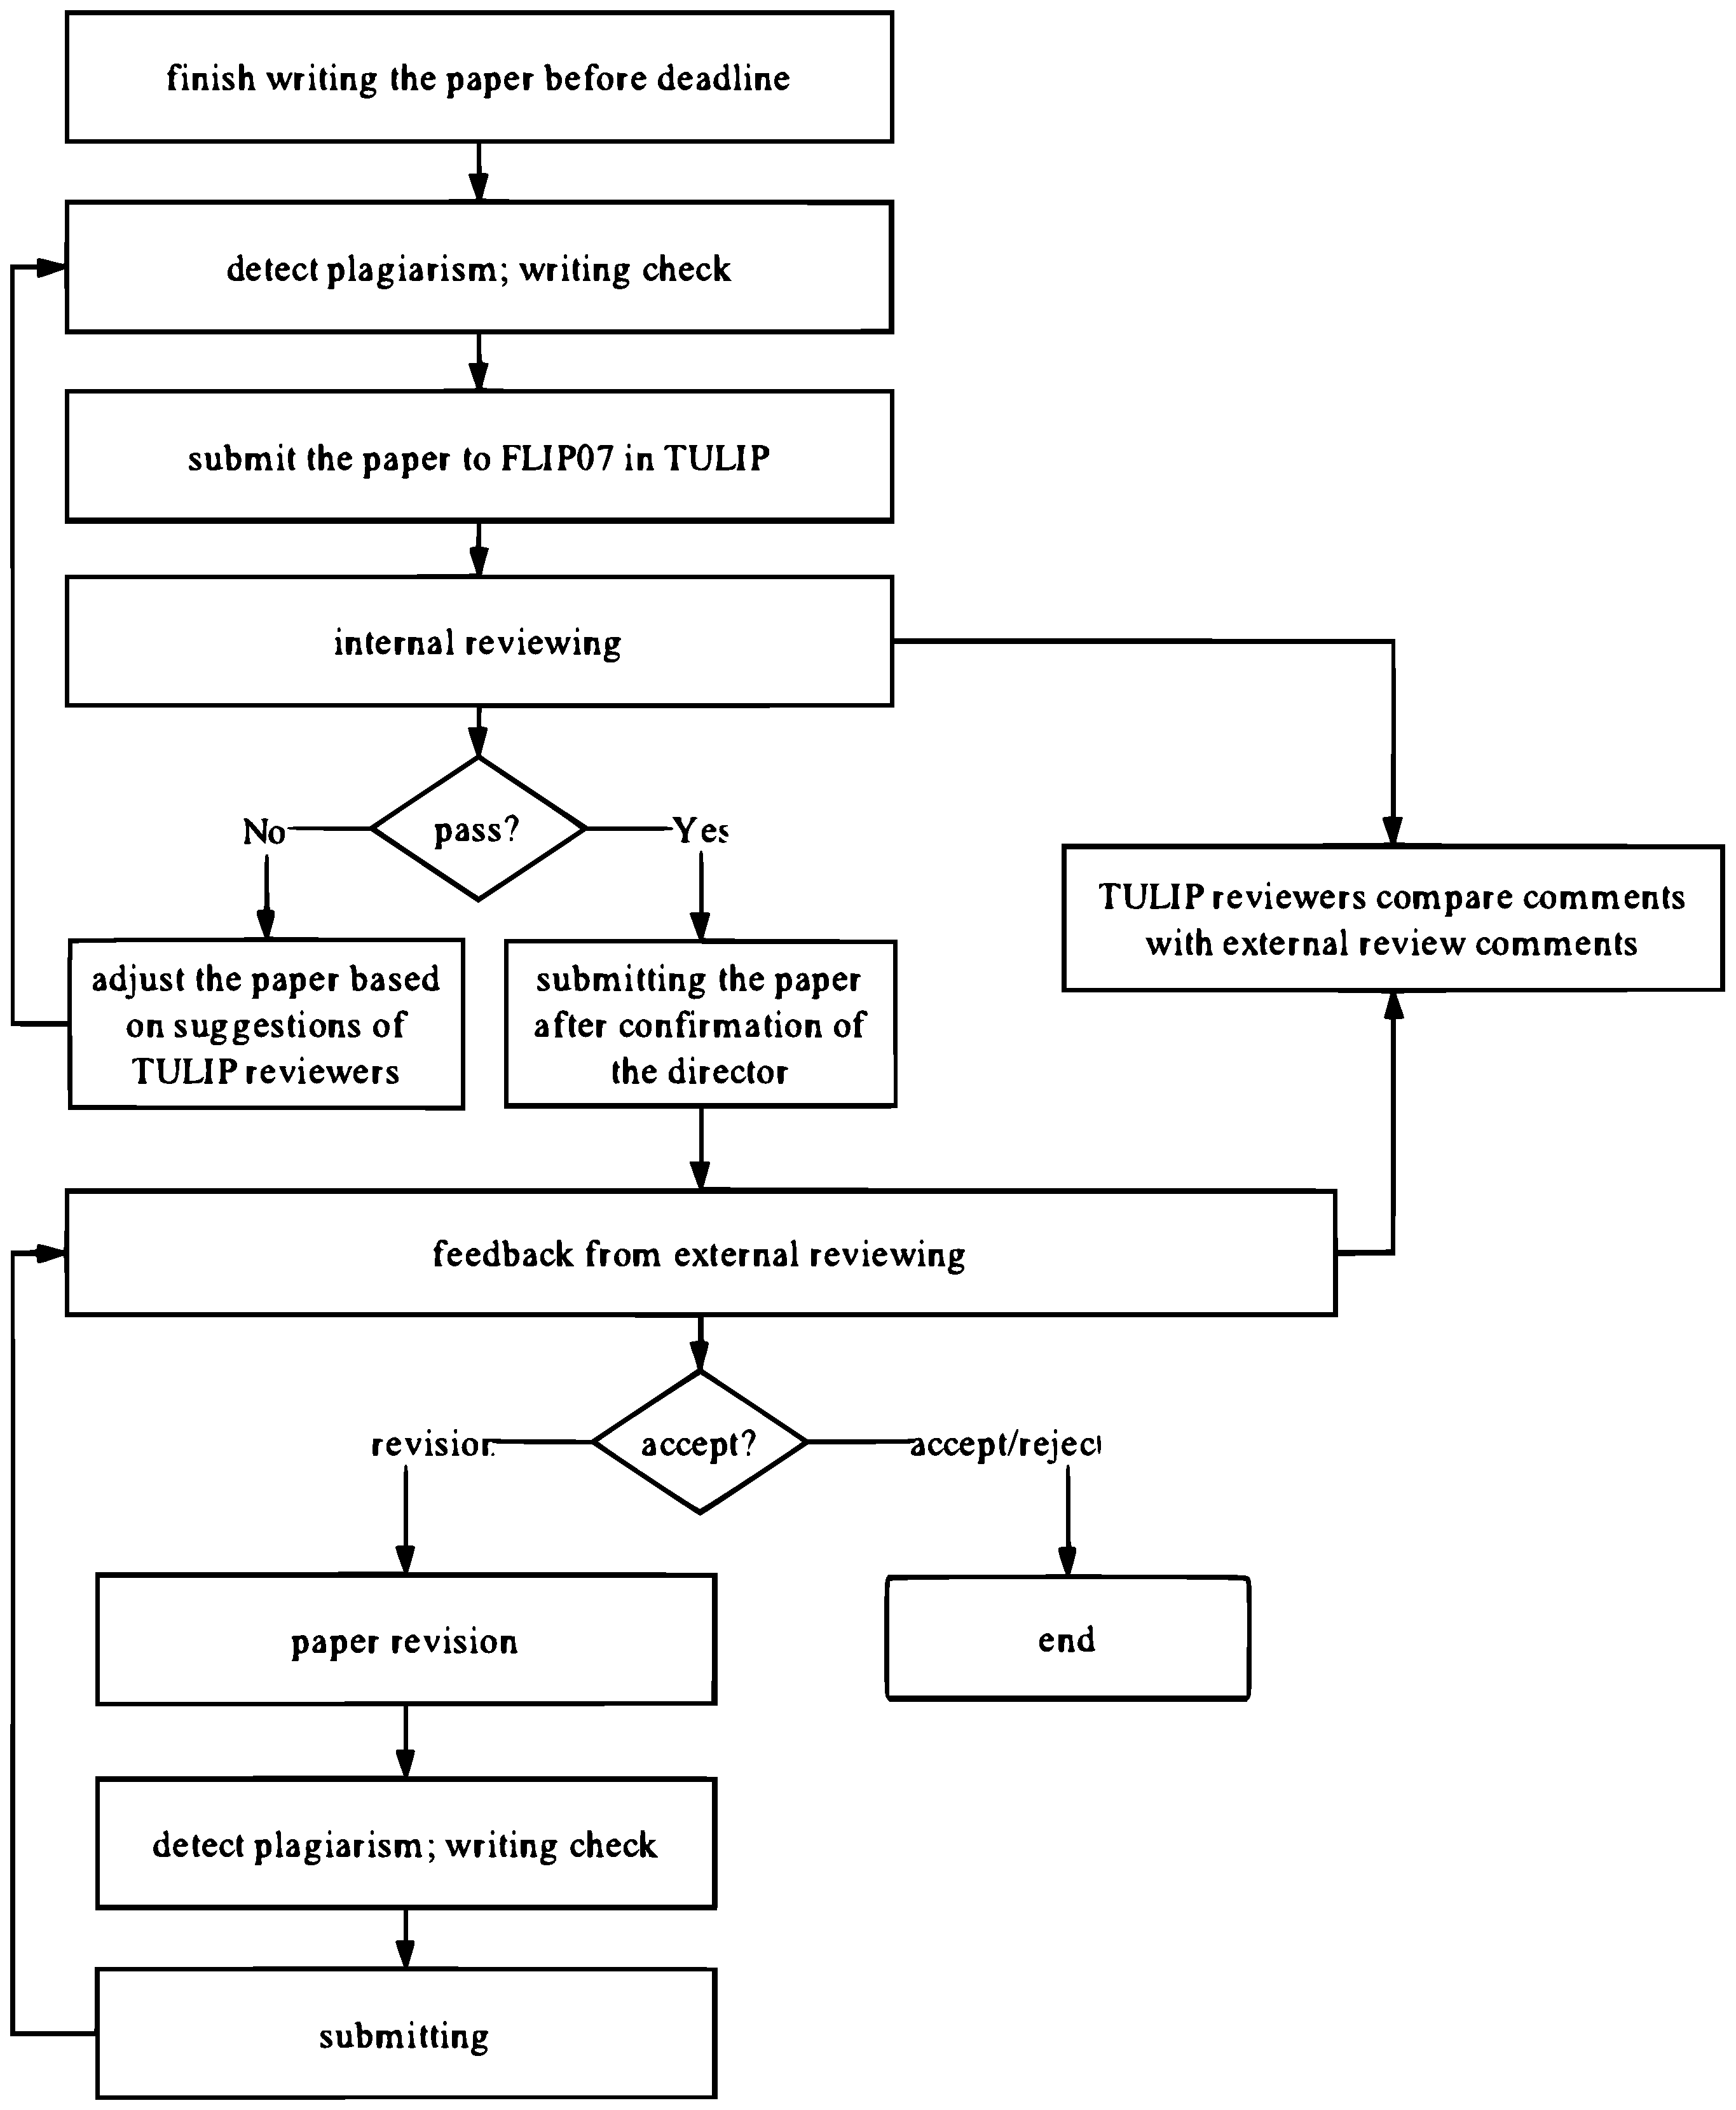
\includegraphics[width=0.47\textwidth]{./figures/writing-skills/submission_procedure.eps}
	% 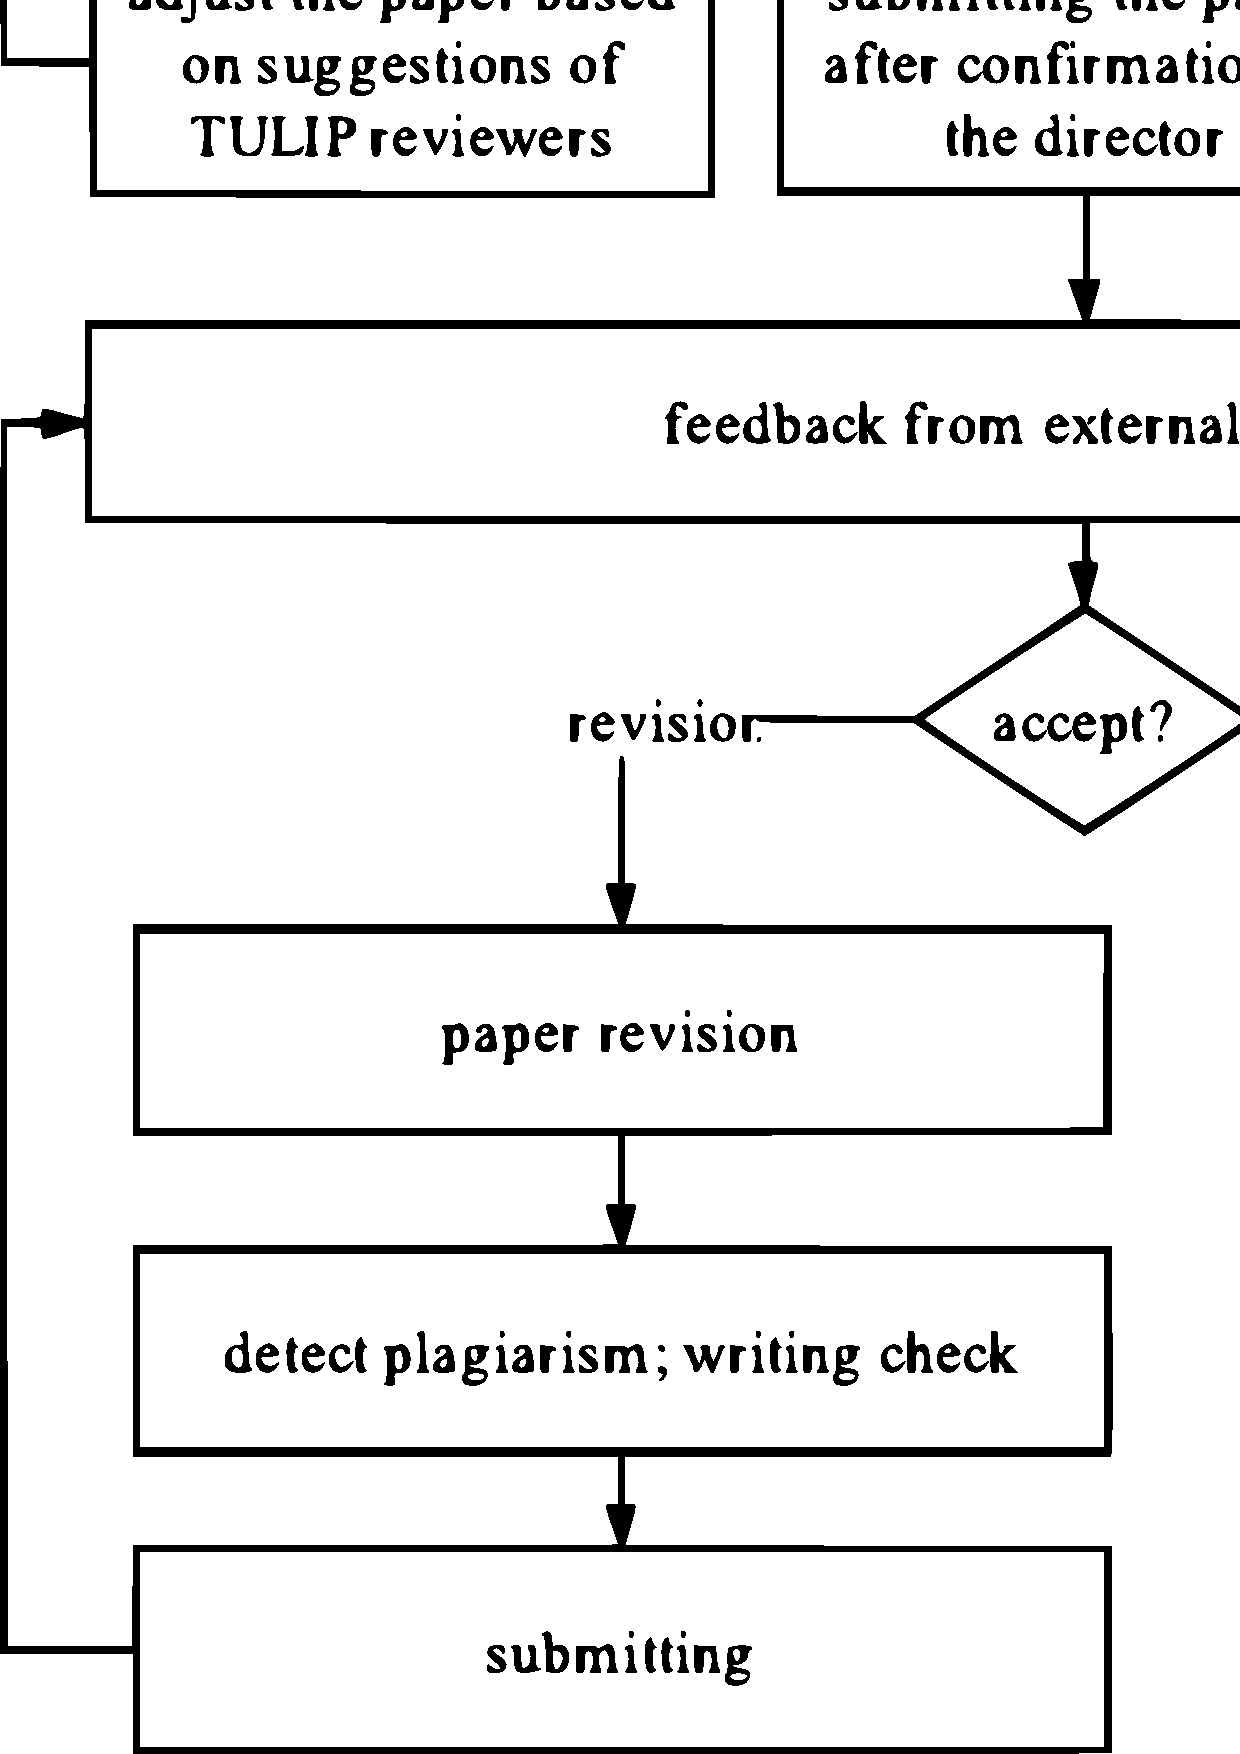
\includegraphics[width=0.5\textwidth,natwidth=610,natheight=642]{./figures/writing-skills/submission_procedure.pdf}
\end{slide}

%%%%%%%%%%%%%%%%%%%%%%%%%%%%%%%%%%%%%%%%%%%%%%%%%%%%%%%%%%%%%%%%%%%%%

%%==========================================================================================
\section{Reference}

%%%%%%%%%%%%%%%%%%%%%%%%%%%%%%%%%%%%%%%%%%%%%%%%%%%%%%%%%%%%%%%%%%%%%

\begin{slide}[toc=,bm=]{Reference}
	\bibliographystyle{plain}
	\nobibliography{tulip-writing}	
	\begin{enumerate}
		\item \bibentry{George}
		\item \bibentry{Yaoqi}
		\item \bibentry{Mike}
		\item \bibentry{Simon}
	\end{enumerate}
\end{slide}

%%%%%%%%%%%%%%%%%%%%%%%%%%%%%%%%%%%%%%%%%%%%%%%%%%%%%%%%%%%%%%%%%%%%

%%==========================================================================================

\end{document}

\endinput
